% --
% Neural Network Architectures

\section{Neural Network Architectures}\label{sec:nn_arch}
\thesisStateNotReady
All neural network architectures evaluated on the Key Word Spotting (KWS) task of speech commands are presented here.
The fundamental architectures types were:
\begin{enumerate}
	\item Convolutional Neural Networks (CNN)
	\item Generative Adversarial Neural Networks (GAN)
	\item Wavenets
\end{enumerate}
CNNs were used for the classification of MFCC features and are therefore the main architecture type within this thesis.
Generative models, such as GANs, were evaluated in regards of their ability to generate samples from the data distribution.
Further the trained weights from the convolutional layers were applied as pre-trained weights for initialisation purpose of a CNN networks with the same convolutional layer structure.
%Wavenets were compared to the CNNs architectures and provide a completely different approach with the use of raw audio samples as inputs features.
A completely different approach to the KWS task was the evaluation of Wavenets, operating on raw audio samples as input features.
In an online system using the Wavenet architecture, no Mel Frequency Cepstral Coefficients (MFCC) have to be extracted, however it will be showed, that the overall computations are not reduced, because the complexity of Wavenets require many operations.

The amount of parameters and operations are provided for each architecutre, to give a comparison between the used models in regards of their computational footprint.


% --
% CNNs

\subsection{Convolutional Neural Networks}\label{sec:nn_arch_cnn}
Three different CNN designs were evaluated, with focus on the striding (shifting) properties of the convolutional filters.
The \texttt{conv-fstride4} model has a kernel size adjusted to the length of the frame (time) dimension of the input features and is therefore striding only in the MFCC (frequency) dimension.
In contrast the \texttt{conv-jim} model has a kernel size adjusted to the feature dimension and therefore strides only in the frame (time) dimension.
Also one traditional model named \texttt{conv-trad} is used, that does the striding of convolutional filters in both dimensions.
The summary of the models is presented as follows:
\begin{itemize}
	\item \texttt{conv-trad}: from \cite{Sainath2015} a traditional CNN network, striding in both dimensions.
	\item \texttt{conv-fstride4}: from \cite{Sainath2015}, striding only in frequency dimension.
	\item \texttt{conv-jim}: self designed model, striding only in frame dimension.
\end{itemize}
The naming of the \texttt{conv-trad} and \texttt{conv-fstride4} comes from their original papers, the self defined network \texttt{conv-jim} was named bluntly after the astronaut avatar, that is used for the deployed video game.
The network architecture of the traditional network (\texttt{conv-trad}) is shown in \rfig{nn_arch_cnn_trad}.
% conv-trad
\begin{figure}[!ht]
  \centering
    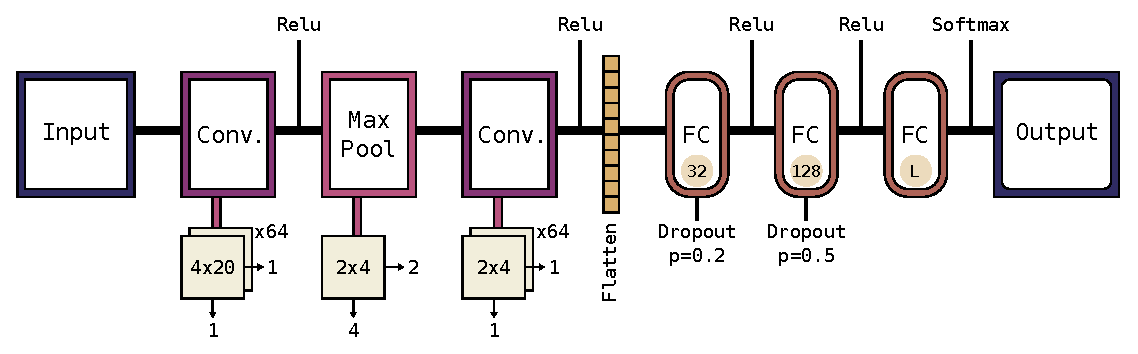
\includegraphics[height=0.2\textwidth]{./4_nn/figs/nn_arch_cnn_trad.eps}
  \caption{Traditional CNN network design from \cite{Sainath2015} named \texttt{conv-trad}.}
  \label{fig:nn_arch_cnn_trad}
\end{figure}
\FloatBarrier
\noindent
The \texttt{conv-trad} network consists of 2 convolutional layers and one max pooling layer in between.
The architecture was adapted from \cite{Sainath2015} as a baseline network and modified a bit in the kernel sizes, so that also reduced input features, for instance 12 MFCCs instead of 39 MFCC (plus deltas and energies), can be computed with the same model.
The length of 20 frames in the first convolutional layer is reasonable and correspond approximately to the length of a vowel sound.
Note that the \enquote{Flatten} layer simply flattens the output tensor of the last convolutional layers to 1-dimension, so that fully-connected (FC) layers can be appended.
Dropout was used in the first two FC layers to improve generalization.
The last FC layer has $L$ nodes corresponding to $L$ output class labels, depending on the amount of chosen key words in the vocabulary.
Assuming that the input will be of shape $d_x = (1 \times 12 \times 50)$ this will give following dimensions and operations as listed in \rtab{nn_arch_cnn_trad}.
\begin{table}[ht!]
\small
\begin{center}
\caption{Network footprint of \texttt{conv-trad} with 12 output labels.}
\begin{tabular}{ M{1.5cm} M{1.4cm} M{1.2cm} M{1.2cm} M{2cm} M{1.8cm} M{2.3cm} }
\toprule
 \textbf{layer types} & \textbf{number of feature maps} & \textbf{kernel size} & \textbf{stride} & \textbf{output dimension} & \textbf{number of parameters} & \textbf{number of operations}\\
\midrule
input & - & - & - & $1 \times 12 \times 50$ & - & -\\
conv. & 64 & $(4 \times 20)$ & $(1, 1)$ & $64 \times 9 \times 31$ & \num{5184} & \SI{2874.82}{\kilo\ops}\\
max pool & - & $(2 \times 4)$ & $(2, 4)$ & $64 \times 4 \times 7$ & - & -\\
conv. & 64 & $(2 \times 4)$ & $(1, 1)$ & $64 \times 3 \times 4$ & \num{32832} & \SI{835.58}{\kilo\ops}\\
flatten & - & - & - & $1 \times 768$ & - & - \\
fc & - & - & - & $1 \times 32$ & \num{24608} & \SI{49.18}{\kilo\ops} \\
fc & - & - & - & $1 \times 128$ & \num{4224} & \SI{8.32}{\kilo\ops} \\
fc & - & - & - & $1 \times 12$ & \num{1548} & \SI{3.08}{\kilo\ops} \\
\midrule
\textbf{sum} & - & - & - & - & \textbf{\num{68396}} & \textbf{\SI{3770.98}{\kilo\ops}} \\ 
\bottomrule
\label{tab:nn_arch_cnn_trad}
\end{tabular}
\end{center}
\vspace{-4mm}
\end{table}
\FloatBarrier
\noindent

The \texttt{conv-fstride4} has the kernel size adapted to the input frame size and is therefore striding only in the frequency dimension.
The kernel heigth of 8 with vertical stride of 4 creates only two dimensions in the vertical direction for an input size of $12 \times 50$, which is very energy efficient. 
The model is shown in \rfig{nn_arch_cnn_fstride} and its footprint is listed in \rtab{nn_arch_cnn_fstride4}
\begin{figure}[!ht]
  \centering
    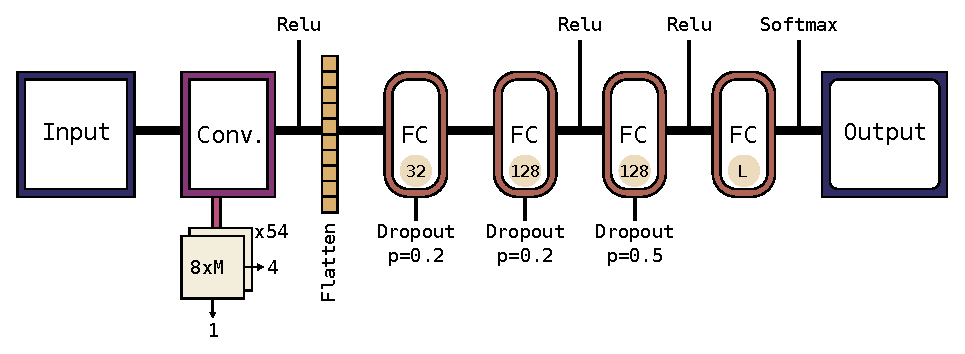
\includegraphics[height=0.2\textwidth]{./4_nn/figs/nn_arch_cnn_fstride.eps}
  \caption{Frequency striding CNN network design from \cite{Sainath2015} named \texttt{conv-fstride4}.}
  \label{fig:nn_arch_cnn_fstride}
\end{figure}
\FloatBarrier
\noindent
\begin{table}[ht!]
\begin{center}
\caption{Network footprint of \texttt{conv-fstride4} with 12 output labels.}
\begin{tabular}{ M{1.5cm} M{1.5cm} M{1.4cm} M{1.4cm} M{2cm} M{2.5cm} M{2.5cm} }
\toprule
 \textbf{layer types} & \textbf{number of feature maps} & \textbf{kernel size} & \textbf{stride} & \textbf{output dimension} & \textbf{number of operations}\\
\midrule
input & - & - & - & $1 \times 12 \times 50$ & -\\
conv. & 54 & $(8 \times 50)$ & $(4, 1)$ & $54 \times 2 \times 1 $ & \SI{86.51}{\kilo\ops}\\
flatten & - & - & - & $1 \times 108$ & - \\
fc & - & - & - & $1 \times 32$ & \SI{6.94}{\kilo\ops} \\
fc & - & - & - & $1 \times 128$ & \SI{8.32}{\kilo\ops} \\
fc & - & - & - & $1 \times 128$ & \SI{32.90}{\kilo\ops} \\
fc & - & - & - & $1 \times 12$ & \SI{3.08}{\kilo\ops} \\
\midrule
\textbf{sum} & - & - & - & - & \textbf{\SI{137.75}{\kilo\ops}} \\ 
\bottomrule
\label{tab:nn_arch_cnn_fstride4}
\end{tabular}
\end{center}
\vspace{-4mm}
\end{table}
\FloatBarrier
\noindent
The self designed \texttt{conv-jim} consists of two convolutional layers, where the first has an adaptive kernel size in the feature (frequency) dimension and is therefore striding only in frame (time) dimension.
The kernel width of the first convolutional filters is set to $20$, which illustrates much of the learned data structure in the feature maps after the training.
The second convolutional filter has a width of $5$ intended for temporal variations.
The \texttt{conv-jim} model is shown in \rfig{nn_arch_cnn_conv-jim} with footprint in \rtab{nn_arch_cnn_jim}.
\begin{figure}[!ht]
  \centering
    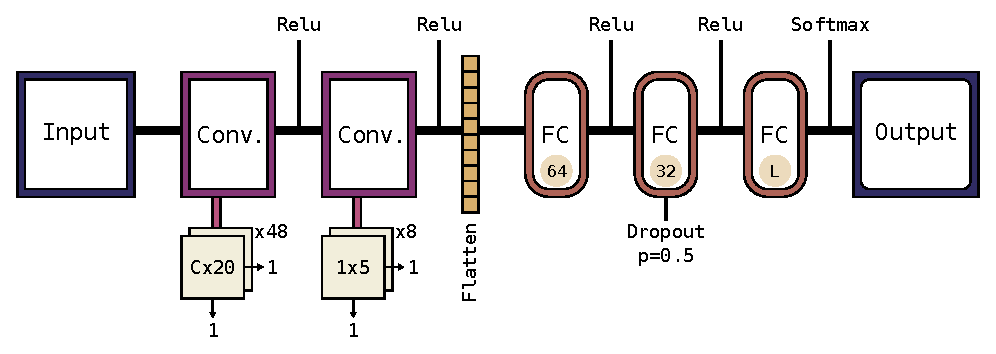
\includegraphics[height=0.2\textwidth]{./4_nn/figs/nn_arch_cnn_conv-jim.eps}
  \caption{Self designed frame (time) striding CNN named \texttt{conv-jim}.}
  \label{fig:nn_arch_cnn_conv-jim}
\end{figure}
\FloatBarrier
\noindent
\begin{table}[ht!]
\small
\begin{center}
\caption{Network footprint of \texttt{conv-jim} with 12 output labels.}
\begin{tabular}{ M{1.5cm} M{1.4cm} M{1.2cm} M{1.2cm} M{2cm} M{1.8cm} M{2.3cm} }
\toprule
 \textbf{layer types} & \textbf{number of feature maps} & \textbf{kernel size} & \textbf{stride} & \textbf{output dimension} & \textbf{number of parameters} & \textbf{number of operations}\\
\midrule
input & - & - & - & $1 \times 12 \times 50$ & -\\
conv. & 48 & $(8 \times 50)$ & $(1, 1)$ & $48 \times 1 \times 31 $ & \num{11520} & \SI{715.73}{\kilo\ops}\\
conv. & 8 & $(8 \times 50)$ & $(1, 1)$ & $8 \times 1 \times 27 $ & \num{1920} & \SI{114.05}{\kilo\ops}\\
flatten & - & - & - & $1 \times 216$ & - \\
fc & - & - & - & $1 \times 64$ & \num{13888} & \SI{27.71}{\kilo\ops} \\
fc & - & - & - & $1 \times 32$ & \num{2080} & \SI{4.13}{\kilo\ops} \\
fc & - & - & - & $1 \times 12$ & \num{396} & \SI{0.78}{\kilo\ops} \\
\midrule
\textbf{sum} & - & - & - & - & \textbf{\num{29804}} & \textbf{\SI{862.40}{\kilo\ops}} \\ 
\bottomrule
\label{tab:nn_arch_cnn_jim}
\end{tabular}
\end{center}
\vspace{-4mm}
\end{table}
\FloatBarrier
\noindent
Note that computational footprint of all three CNN models are different.
The lowest amount of computation needed is in the \texttt{conv-fstride4} network because of its stride jump of 4, the second lowest footprint is given by the \texttt{conv-jim} model.
The \texttt{conv-trad} model has the highest amount of computations, which further increase significantly if more cepstral coefficients are used.


% --
% GANs

\subsection{Generative Adversarial Neural Networks}\label{sec:nn_arch_adv}
Generative Adversarial Neural Networks (GAN), as already mentioned in \rsec{prev_nn_adv} and \rsec{nn_theory_gan} are consisting of two separate neural network architectures, denoted as Discriminator (D) and Generator (G) network.
Being able to transfer the obtained weights from the training of the adversarial models, the target layer parameters of the receiving network must coincide with the adversarial network layer parameters.
The convolutional layer parameters of both D and G can be applied for transfering its weights, even if G performs a convolutional upsampling (transposed convolution) instead of a usual convolution, however it is preferred to use frame-based normalization for the G network, otherwise this might not work well.

The major model tested with adversarial pre-training has the same convolutional layer structure as the \texttt{conv-jim} network and is therefore denoted as \texttt{adv-d-jim} shown in \rfig{nn_arch_adv_d_jim} and \texttt{adv-g-jim} in \rfig{nn_arch_adv_g_jim}.
\begin{figure}[!ht]
  \centering
    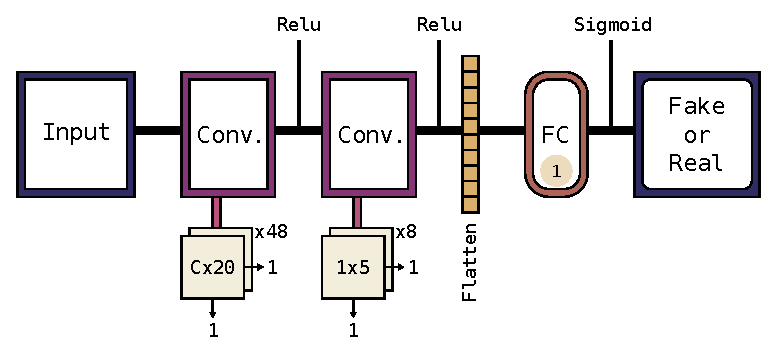
\includegraphics[height=0.2\textwidth]{./4_nn/figs/nn_arch_adv_d_jim.eps}
  \caption{Discriminator network named \texttt{adv-d-jim}.}
  \label{fig:nn_arch_adv_d_jim}
\end{figure}
\FloatBarrier
\noindent
\begin{figure}[!ht]
  \centering
    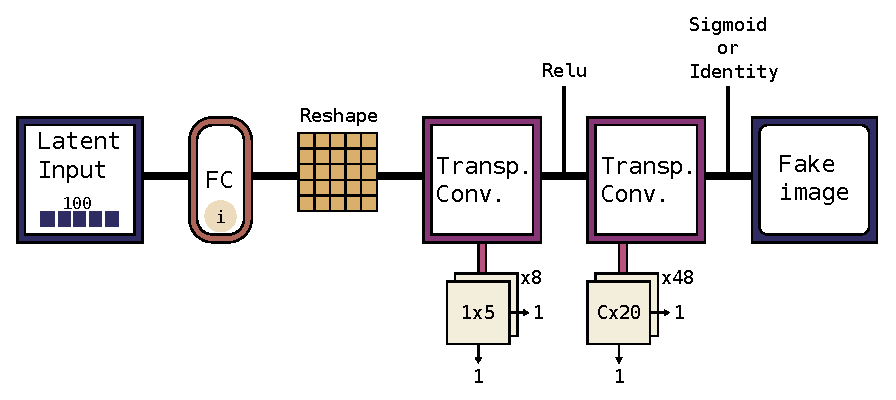
\includegraphics[height=0.23\textwidth]{./4_nn/figs/nn_arch_adv_g_jim.eps}
  \caption{Generator network named \texttt{adv-g-jim}.}
  \label{fig:nn_arch_adv_g_jim}
\end{figure}
\FloatBarrier
\noindent
Note that the number of operations are the same as in \rtab{nn_arch_cnn_jim}, except for the fully-connected layers.
The \texttt{adv-g-jim} model uses either the sigmoid or an identity (same output as input) activation function, depending whether the Mel Frequency Cepstral Coefficients (MFCC) are frame-based normalized or not.
If the MFCC are frame-based normalized the sigmoid activation function is used to produce outputs in the range of $[0, 1]$, which enhances the models training speed compared to the generation of samples that are not normalized.
%An overview of all models is shown in \rtab{nn_arch_overview} with abbreviations in \rtab{nn_arch_abbreviation}.
%\begin{table}[ht!]
\begin{center}
\caption{Network Architectures Abbreviations}
\begin{tabular}{ M{2.5cm}  M{10cm} }
\toprule
\textbf{Abbreviations} & \textbf{Meaning}\\
\midrule
c[0-9] & convolutional layer with layer number\\
f[0-9] & feed forward fully connected layer with layer number\\
m[0-9] & max pooling layer layer with layer number\\
ch & input channel number for mfccs it is usually 1\\
fs & frame size (usually 50 -> 50ms)\\
ms & feature size (mfcc), depends on feature selection\\
cf & output number of last flattened convolutional layer\\
cl & number of class labels\\
\bottomrule
\label{tab:nn_arch_abbreviation}
\end{tabular}
\end{center}
\vspace{-4mm}
\end{table}
\FloatBarrier
\noindent
%\begin{table}[ht!]
\begin{center}
\caption{Network Architectures Overview with reference names}
\begin{tabular}{ M{2.5cm}  M{2.1cm}  M{2.1cm} M{2.1cm} M{2.5cm}}
\toprule
%\multicolumn{4}{c}{\textbf{Feature Groups}} & \multicolumn{2}{c}{\textbf{Accuracy}} \\
\textbf{Reference name} & \textbf{Feature maps} & \textbf{Kernel sizes} & \textbf{Strides} & \textbf{Feed Forward} \\
\midrule
conv-trad & c1: (ch, 64) c3: (64, 64) & c1: (4, 20) m2: (2, 4) c3: (2, 4) & c1: (1, 1) m2: (2, 4) c3: (1, 1) & f4: (cf, 32) \quad f5: (32, 128) f6: (128, cl)\\
\midrule
conv-fstride & c1: (ch, 54) & c1: (8, fs) & c1: (4, 1) & f2: (cf, 32) \quad f3: (32, 128) \quad f4: (128, 128) \quad f5: (128, cl)\\
\midrule
conv-encoder-fc1 & c1: (ch, 48) \quad c2: (48, 8) & c1: (ms, 20) \quad c2: (1, 5) & c1: (1, 1) \quad c2: (1, 1) & f3: (cf, cl)\\
\midrule
conv-encoder-fc3 & c1: (ch, 48) \quad c2: (48, 8) & c1: (ms, 20) \quad c2: (1, 5) & c1: (1, 1) \quad c2: (1, 1) & f3: (cf, 64) \quad f4: (64, 32) \quad f5: (32, l)\\
\midrule
adv-d-label & c1: (ch, 8) \quad c2: (8, 8) & c1: (ms, 20) \quad c2: (1, 5) & c1: (1, 1) \quad c2: (1, 1) & f3: (cf, 1)\\
\midrule
adv-g-label & c2: (8, 8) \quad c3: (8, ch) & c2: (1, 5) \quad c3: (ms, 20) & c2: (1, 1) \quad c3: (1, 1) & f1: (100, cf)\\
\bottomrule
\label{tab:nn_arch_overview}
\end{tabular}
\end{center}
\vspace{-4mm}
\end{table}
\FloatBarrier
\noindent


% --
% wavenets

\subsection{Wavenets}\label{sec:nn_arch_wavenet}
Wavenets were introduced in \cite{Oord2016} intended for speech generation on the processing of raw audio data.
In the paper it is mentioned that Wavenets can be used for Automatic Speech Recognition (ASR) tasks as well, though it is very sparsely described.
An implementation of a Wavenet can be found in \cite{Herrmann2018} (without class predictions) and motivated the following model structure.
A Wavenet residual block with an extension for class prediction is illustrated in \rfig{nn_arch_wavenet_block}.
\begin{figure}[!ht]
  \centering
    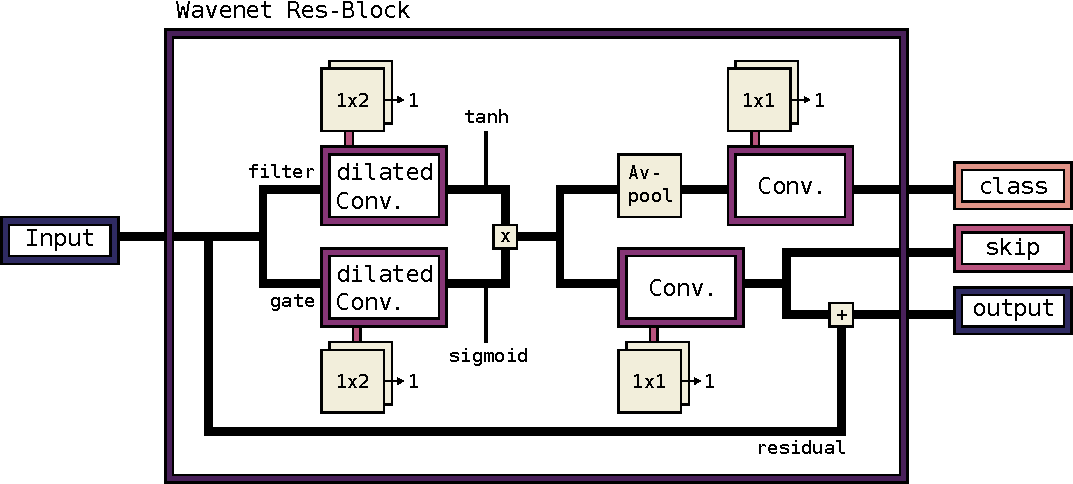
\includegraphics[width=0.7\textwidth]{./4_nn/figs/nn_arch_wavenet_block.eps}
  \caption{Wavenet residual block \cite{Oord2016} with an extension of class prediction layers.}
  \label{fig:nn_arch_wavenet_block}
\end{figure}
\FloatBarrier
\noindent
It is important to note, that the convolutional layers in the residual blocks should not use a bias term, because of bad training results.
One residual block incorporates few parameters, but a huge amount of operations, which are listed in \rtab{nn_arch_wavenet_block}.
\begin{table}[ht!]
\begin{center}
\caption{Residual block of a Wavenet architecture with extension of class predictions and input sample length of 8000.}
\begin{tabular}{ M{1.5cm} M{1.5cm} M{1.4cm} M{1.4cm} M{2cm} M{2.5cm} M{2.5cm} }
\toprule
 \textbf{layer types} & \textbf{number of feature maps} & \textbf{kernel size} & \textbf{stride} & \textbf{output dimension} & \textbf{number of operations}\\
\midrule
input & - & - & - & $1 \times 8000$ & -\\
conv. gate & 16 & $(1 \times 2)$ & $(1, 1)$ & $16 \times 1 \times 8000 $ & \SI{715.73}{\kilo\ops}\\
conv. filter & 16 & $(1 \times 2)$ & $(1, 1)$ & $16 \times 1 \times 8000 $ & \SI{715.73}{\kilo\ops}\\

\midrule
\textbf{sum} & - & - & - & - & \textbf{\SI{862.40}{\kilo\ops}} \\ 
\bottomrule
\label{tab:nn_arch_wavenet_block}
\end{tabular}
\end{center}
\vspace{-4mm}
\end{table}
\FloatBarrier
\noindent
Note that the dilated convolutional filters have a filter size of two with adjustable dilation parameter and that strides are merely done in the time dimension, because the input is a one-dimensional time signal.
The $1 \times 1$ convolutions are a special type of convolutional filters, that work in the same manner as usual convolutions, just with a filter size of one. 
The whole Wavenet architecture is composed of several consecutive Wavenet residual blocks with increasing dilation parameters for the first two convolutional layers (filter and gate).
The whole Wavenet architecture adaption with class prediction is shown in \rfig{nn_arch_wavenet_all}.
\begin{figure}[!ht]
  \centering
    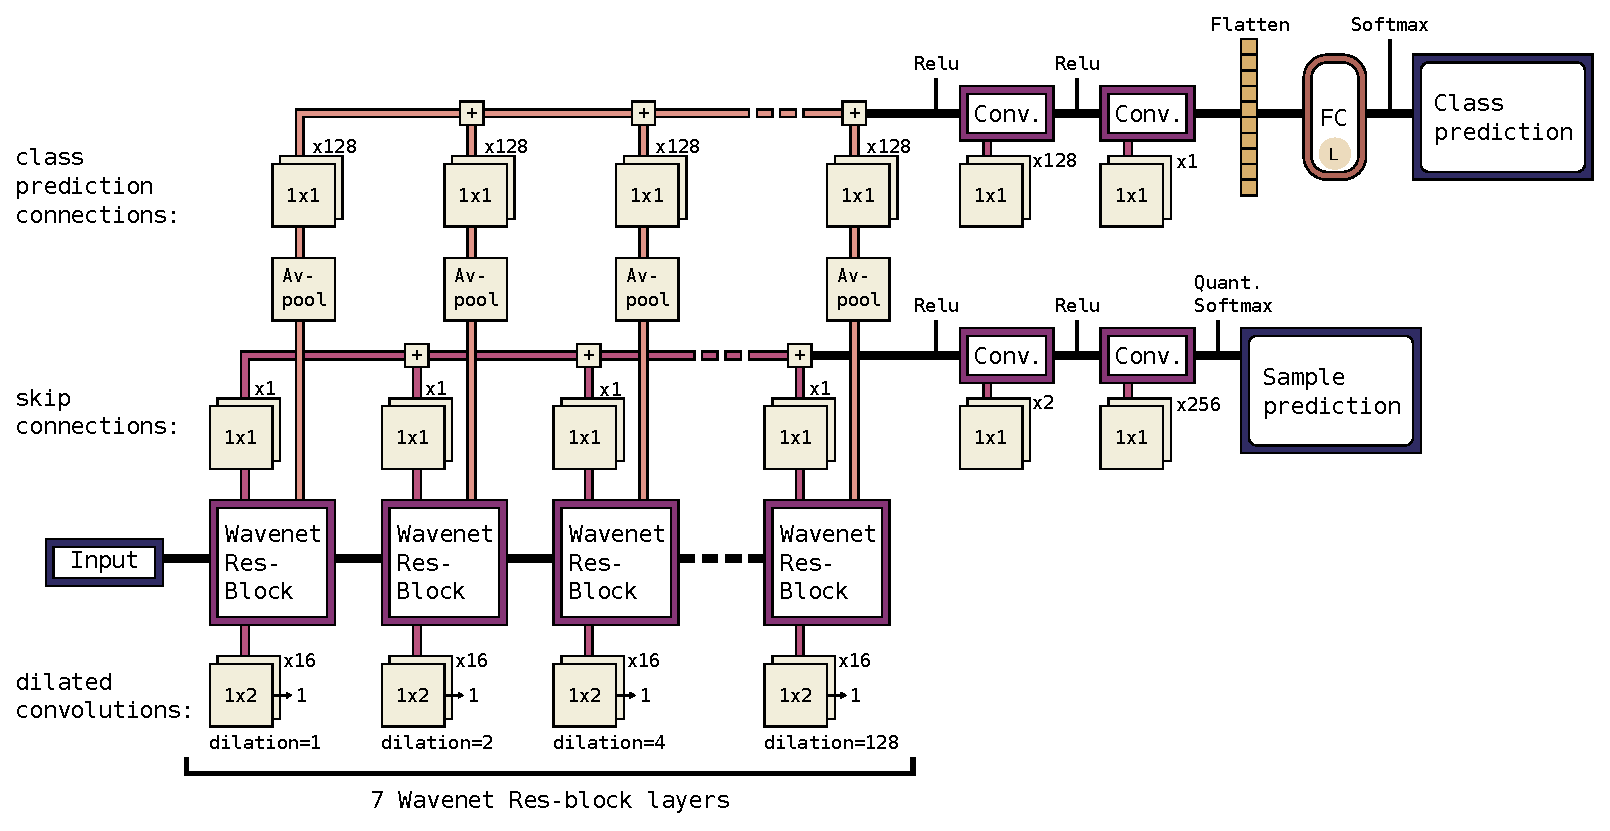
\includegraphics[width=0.9\textwidth]{./4_nn/figs/nn_arch_wavenet_all.eps}
  \caption{Wavenet architecture with class prediction extension.}
  \label{fig:nn_arch_wavenet_all}
\end{figure}
\FloatBarrier
\noindent
Note that the last convolutional layer for the sample prediction has a total amount of feature maps ($1 \times 1$) selected to the quantized audio representation.
More details about the quantization technique used is described in \cite{Oord2016}.
The computational footprint of the whole Wavenet model is listed in \rtab{nn_arch_wavenet_whole}.
\begin{table}[ht!]
\small
\begin{center}
\caption{Whole Wavenet architecture with extension of a class predictions of 12 output labels and input sample length of \num{8000}.}
%\begin{tabular}{ M{2cm} M{1.5cm} M{1.2cm} M{1.2cm} M{2cm} M{1.5cm} M{2.3cm} }
\begin{tabular}{ M{1.5cm} M{1.4cm} M{1.1cm} M{1.1cm} M{2cm} M{1.5cm} M{2.6cm} }
\toprule
 \textbf{Layer Types} & \textbf{Number of Feature Maps} & \textbf{Kernel Size} & \textbf{Stride} & \textbf{Output Dimension} & \textbf{Number of Parameters} & \textbf{Number of Operations}\\
\midrule
input & - & - & - & $1 \times 8000$ & - & -\\
7 res. blocks & - & - & - & - & \num{14896} & \SI{19453.98}{\kilo\ops}\\
conv. s1 & 2 & $(1 \times 1)$ & $(1, 1)$ & $1 \times 1 \times 8000$ & \num{4} & \SI{48.00}{\kilo\ops} \\
conv. s2 & 256 & $(1 \times 1)$ & $(1, 1)$ & $256 \times 1 \times 8000$ & \num{768} & \SI{12288.00}{\kilo\ops} \\
conv. c1 & 128 & $(1 \times 1)$ & $(1, 1)$ & $1 \times 1 \times 99$ & \num{16512} & \SI{4866.05}{\kilo\ops} \\
conv. c2 & 1 & $(1 \times 1)$ & $(1, 1)$ & $1 \times 1 \times 99$ & \num{129} & \SI{38.02}{\kilo\ops} \\
fc & - & - & - & $1 \times 12$ & \num{1200} & \SI{2.39}{\kilo\ops} \\
\midrule
\textbf{sum} & - & - & - & - & \textbf{\num{33509}} & \textbf{\SI{36695.02}{\kilo\ops}} \\
\bottomrule
\label{tab:nn_arch_wavenet_whole}
\end{tabular}
\end{center}
\vspace{-4mm}
\end{table}
\FloatBarrier
\noindent

